%%%%%%%%%%%%%%%%%%%%%%%%%%%%% DEFAULT TEXT FILE %%%%%%%%%%%%%%%%%%%%%%%%%%%%%
\documentclass[12pt,a4paper]{article}
\usepackage[utf8]{inputenc}             % Default unicode
\usepackage{hyperref}
%\usepackage[none]{hyphenat}             % Disables wordbreak
%\usepackage{multicol}                  % multiple columns

%\usepackage{libertine}                 % font
%\renewcommand{\familydefault}{\sfdefault}
%\usepackage{changepage}

%%%%%%%%%%%%%%%%%%%%%%%%%%%%%% DOCUMENT LAYOUT %%%%%%%%%%%%%%%%%%%%%%%%%%%%%%
\usepackage{geometry}
\usepackage{svg}
\geometry{
%    a4paper,
%    total={170mm,257mm},
%    left=20mm,
%    top=20mm,
    headheight=16pt,
    margin=1in
}


%\usepackage[explicit]{titlesec}
%\newcommand{\raisedrulefill}[2][0ex]{\leaders\hbox{\rule[#1]{0.1pt}{#2}}\hfill}
%\titleformat{\subsection}{\Large\bfseries}{\thesubsection. }{0em}{#1\,\raisedrulefill[0ex]{1pt}}

%%%%%%%%%%%%%%%%%%%%%%%%%%%%% IMAGES & GRAPHICS %%%%%%%%%%%%%%%%%%%%%%%%%%%%%
\usepackage{graphicx}                      % images
\graphicspath{ {../screenshots} }

\usepackage{fontawesome}     %\faicon      % icons


%\usepackage{pifont}    %\ding{118}         % symbols

%\usepackage{tikz}                           % graphics
%\usetikzlibrary{shapes.geometric, arrows}

% Create normal bullet point using $\bigcdot$
%\makeatletter
%\newcommand*\bigcdot{\mathpalette\bigcdot@{.7}}
%\newcommand*\bigcdot@[2]{\mathbin{\vcenter{\hbox{\scalebox{#2}{$\m@th#1\bullet$}}}}}
%\makeatother

%%%%%%%%%%%%%%%%%%%%%%%%%%%%%%%% MATH SYNTAX %%%%%%%%%%%%%%%%%%%%%%%%%%%%%%%%
%\usepackage{amsmath, amssymb}

%%%%%%%%%%%%%%%%%%%%%%%%%%%%%%%% PROGRAMMING %%%%%%%%%%%%%%%%%%%%%%%%%%%%%%%%
\usepackage{listings,xcolor}
\definecolor{backcolour}{rgb}{0.95,0.95,0.95}
\definecolor{dkgreen}{rgb}{0,0.6,0}
\definecolor{gray}{rgb}{0.5,0.5,0.5}
\definecolor{mauve}{rgb}{0.58,0,0.82}
\definecolor{darkerblue}{HTML}{010161}

\lstdefinestyle{python}{
    language=Python,
    showstringspaces=false,
    columns=flexible,
    basicstyle=\ttfamily\footnotesize,
    numbers=none,                    
    backgroundcolor=\color{backcolour},   
    numberstyle=\tiny\color{gray},
    keywordstyle=\color{blue},
    commentstyle=\color{dkgreen},
    stringstyle=\color{mauve},
    keepspaces=false,                 
    numbersep=5pt,                  
    showspaces=false,                
    showstringspaces=false,
    breaklines=true,
    breakatwhitespace=false,
    tabsize=2,
%    xleftmargin=\parindent
%    number=none
}

\usepackage{fancyhdr}
\pagestyle{fancy}
\fancyhf{}
\fancyhead[L]{\color{darkerblue} Discrete Structures II}
\fancyhead[C]{}
\fancyhead[R]{\color{darkerblue} \partname{} \thepart{}}
\fancyfoot[L]{}
\fancyfoot[C]{\thepage}
\fancyfoot[R]{}
% Remove the line in the header
\renewcommand{\headrulewidth}{0pt}
%\renewcommand{\footrulewidth}{0.4pt}

%%%%%%%%%%%%%%%%%%%%%%%%% TABLE OF CONTENTS SETTINGS %%%%%%%%%%%%%%%%%%%%%%%%
%\usepackage{titletoc, tocloft}
%\renewcommand{\cftpartleader}{\cftdotfill{\cftdotsep}}  % for parts
%\renewcommand\thepart{\arabic{part}}                    % number system
%\setlength{\cftsecindent}{1cm}                          % indent section
\renewcommand{\contentsname}{\Huge\bfseries Table of Contents}

%%%%%%%%%%%%%%%%%%%%%%%%%%%%%%%%%%%%%%%%%%%%%%%%%%%%%%%%%%%%%%%%%%%%%%%%%%%%%
%%%%%%%%%%%%%%%%%%%%%%%%%%%%%%%%%% DOCUMENT %%%%%%%%%%%%%%%%%%%%%%%%%%%%%%%%%
\begin{document}
%%%%%%%%%%%%%%%%%%%%%%%%%%%%%%%%%%% TITLE %%%%%%%%%%%%%%%%%%%%%%%%%%%%%%%%%%%
\thispagestyle{empty}
\addcontentsline{toc}{part}{Title page}
\pagenumbering{roman}

\vspace*{\fill}
\begingroup
\centering

    \textbf{POLYTECHNIC UNIVERSITY OF THE PHILIPPINES\\
    BACHELOR OF SCIENCE IN COMPUTER SCIENCE}\vspace{.1in}

\noindent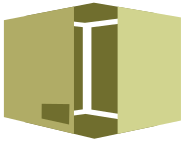
\includegraphics[width=3in,height=3in]{logo.png}\vspace{.1in}

    \textbf{DISCRETE STRUCTURES II}\vspace{.1in}
    
    \textbf{
        \huge Invento Management System Documentation
    }\vspace{2in}

\endgroup
\vspace*{\fill}

    \noindent\textbf{BSCS 2-1N\\Group 3}\vspace{0.2in}

    \noindent
    \begin{tabular}{l l}
        \textbf{Project Manager:} & Annalyn Belen \\
        \textbf{Designer:} & Monika Jea Ng\\
        \textbf{Developer:} & Steve Pabular \\
        \textbf{Systems Analyst:} & John Nicolas Oandasan\\
        \textbf{Business Analyst:} & Hazel Conception\\
        \textbf{Technical Writer:} & Percian Cayaban
    \end{tabular}\vspace{0.2in}

    \noindent\textbf{Instructor:} Prof. Angie Payne

\newpage
%%%%%%%%%%%%%%%%%%%%%%%%%%%%% TABLE OF CONTENTS %%%%%%%%%%%%%%%%%%%%%%%%%%%%%
\thispagestyle{plain}
\addcontentsline{toc}{part}{Contents}
\tableofcontents
\newpage
%%%%%%%%%%%%%%%%%%%%%%%%%%%%%%%%%% CONTENT %%%%%%%%%%%%%%%%%%%%%%%%%%%%%%%%%%
\pagenumbering{arabic}
\setcounter{page}{1}
\part{ Invento Management System }

\section*{Description \hrulefill}
\addcontentsline{toc}{section}{Description}
    \begin{itemize}
        \item This program is an inventory system which is simple and easy to use.
        \item Designed to calculate products currently present in the inventory and quantities.
        \item Monitors inventory changes and sales performance in at most, the past week.
    \end{itemize}
\hrulefill

\section*{Setup}
\addcontentsline{toc}{section}{Setup}

This program requires the 3.10+ version of Python installed and the following packages:

\begin{itemize}
    \item \texttt{customtkinter}
    \item \texttt{Pillow}
    \item \texttt{matplotlib}
\end{itemize}

\noindent Which can be installed with the following command:

\hfill{}

\texttt{pip install --upgrade customtkinter Pillow matplotlib}

\hfill{}

\noindent There also is a detailed setup guide available at \href{https://github.com/steguiosaur/invento}{\textcolor{blue}{https://github.com/steguiosaur/invento}} .

\newpage
\section*{Execution}
\addcontentsline{toc}{section}{Execution}

\hspace\parindent The program can be executed by using the command \texttt{python Main.py} in a terminal. If there aren't any dependency conflicts and logged-in session, it would show the Login page (shown in Figure \ref{fig:login}) wherein it takes an input for the current registered accounts.

\hfill{}

\begin{figure}[ht]
  \centering
  \includegraphics[width=5in,height=3in]{Login.png}
  \caption{Login page}
  \label{fig:login}
\end{figure}

\hspace\parindent
On this page (Figure \ref{fig:register}), you could register a new account by entering the required information.

\hfill{}

\begin{figure}[ht]
  \centering
  \includegraphics[width=5in,height=3in]{Register.png}
  \caption{Register page}
  \label{fig:register}
\end{figure}

\newpage

\part{ Instruction Manual }
\section{Main.py}

\section{Utils Package}

    \subsection{accounts.py}

    \subsection{assets.py}

\section{Customwidget}

\section{Pages}

\section{Tabs}

%%%%%%%%%%%%%%%%%%%%%%%%%%%%%%%%%%%% END %%%%%%%%%%%%%%%%%%%%%%%%%%%%%%%%%%%%
\end{document}
%%%%%%%%%%%%%%%%%%%%%%%%%%%%%%%%%%%%%%%%%%%%%%%%%%%%%%%%%%%%%%%%%%%%%%%%%%%%%


%%%%%%%%%%%%%%%%%%%%%%%%%%%%%%%%%%% GUIDE %%%%%%%%%%%%%%%%%%%%%%%%%%%%%%%%%%%
%%%%%%%%%%%%%%%%%%%%%%%%%%%%%%%% IMAGE
%\includegraphics[width=\textwidth,height=4.5in]{image.png}
%
%%%%%%%%%%%%%%%%%%%%%%%%%%%%%%%% PROGRAMMING
%\begin{listings}[style=Java]
%    ... code
%\end{listings}
%
%%%%%%%%%%%%%%%%%%%%%%%%%%%%%%% TABLE
%\begin{tabular}{c c c}
%    text & text & text
%\end{tabular}
%
%%%%%%%%%%%%%%%%%%%%%%%%%%%%%%% MINIPAGE
%\begin{minipage}[t]{50pt}
%    \flushleft
%\end{minipage}
